%%%%%%%%%%%%%%%%%%%%%%%%%%%%%%%%%%%%%%%%%%%%%%%%%%%%%%%%%%%%%%%%%%%%%%
% How to use writeLaTeX: 
%
% You edit the source code here on the left, and the preview on the
% right shows you the result within a few seconds.
%
% Bookmark this page and share the URL with your co-authors. They can
% edit at the same time!
%
% You can upload figures, bibliographies, custom classes and
% styles using the files menu.
%
%%%%%%%%%%%%%%%%%%%%%%%%%%%%%%%%%%%%%%%%%%%%%%%%%%%%%%%%%%%%%%%%%%%%%%

\documentclass[12pt]{article}

\usepackage{sbc-template}

\usepackage[round]{natbib}

\usepackage{indentfirst}
\usepackage{epigraph}

\usepackage{graphicx,url}

\usepackage[brazil]{babel}   
\usepackage[utf8]{inputenc}

\usepackage{verbatim}

\usepackage{color}
    \definecolor{lightgray}{rgb}{0.95, 0.95, 0.95}
    \definecolor{darkgray}{rgb}{0.4, 0.4, 0.4}
    \definecolor{purple}{rgb}{0.65, 0.12, 0.82}
    \definecolor{ocherCode}{rgb}{1, 0.5, 0} % #FF7F00 -> rgb(239, 169, 0)
    \definecolor{blueCode}{rgb}{0, 0, 0.93} % #0000EE -> rgb(0, 0, 238)
    \definecolor{greenCode}{rgb}{0, 0.6, 0} % #009900 -> rgb(0, 153, 0) 

\usepackage{listings}
\lstdefinelanguage{HTML5}{
    sensitive=true,
    keywords={%
    % JavaScript
    typeof, new, true, false, catch, function, return, null, catch, switch, var, if, in, while, do, else, case, break,
    % HTML
    html, title, meta, style, head, body, script, div,
    % CSS
    border:, transform:, -moz-transform:, transition-duration:, transition-property:,
    transition-timing-function:
    },
    % https://texblog.org/tag/otherkeywords/
    otherkeywords={<, >, \/},   
    ndkeywords={class, export, boolean, throw, implements, import, this},   
    comment=[l]{//},
    % morecomment=[s][keywordstyle]{<}{>},  
    morecomment=[s]{/*}{*/},
    morecomment=[s]{<!}{>},
    morestring=[b]',
    morestring=[b]",    
    alsoletter={-},
    alsodigit={:}
}
\lstset{%
    % Basic design
    backgroundcolor=\color{lightgray},
    basicstyle={\small\ttfamily},   
    frame=l,
    % Line numbers
    xleftmargin={0.75cm},
    numbers=left,
    stepnumber=1,
    firstnumber=1,
    numberfirstline=true,
    % Code design
    identifierstyle=\color{black},
    %keywordstyle=\color{blue}\bfseries,
    %ndkeywordstyle=\color{greenCode}\bfseries,
    %stringstyle=\color{ocherCode}\ttfamily,
    %commentstyle=\color{darkgray}\ttfamily,
    % Code
    language={HTML5},
    tabsize=2,
    showtabs=false,
    showspaces=false,
    showstringspaces=false,
    extendedchars=true,
    breaklines=true
}

\usepackage[table]{xcolor}
\usepackage{multirow}
\usepackage{scalefnt}
\usepackage{enumerate}
\usepackage{hyperref}     
\usepackage{array}

\usepackage{tikz}
\usetikzlibrary{shapes,arrows}
\usetikzlibrary{positioning}
     
\sloppy

%\title{API \emph{Web} de Geovisualização para Tratamento e Análise de Dados Espaciais}
\title{GeoMap BR: API \emph{Web} de Geovisualização para Análise Espacial de Dados do Território Brasileiro }
%\title{API \emph{Web} de Geovisualização para Análise Espacial de Dados do Território Brasileiro}

%\author{Yuri H. Martins\inst{1}, Ivre Marjorie R. Machado\inst{1}}
\author{Yuri H. Martins\inst{1}, Kleber Jacques F. de Souza\inst{1}}
%\author{Yuri H. Martins\inst{1}, Ivre Marjorie R. Machado\inst{1}, Kleber Jacques F. de Souza\inst{1}}
\address{PUC Minas em Contagem\\Bacharelado em Sistemas de Informação
%\email{yurihm@hotmail.com, ivre.marjorie@gmail.com}
\email{yurihm@hotmail.com, klebersouza@pucminas.br}
%\email{yurihm@hotmail.com, ivre.marjorie@gmail.com, klebersouza@pucminas.br}
}

\begin{document} 

\maketitle

\begin{resumo} 

A análise visual de dados é uma forma simplificada de se obter informações específicas e centralizadas referente a uma grande massa de dados. A geovisualização, como sendo uma vertente deste assunto, se tornou uma poderosa ferramenta que auxilia na tomada de decisão para resolução de diversos tipos de problemas de grandeza espacial. Sendo assim, o objetivo deste trabalho é prover uma ferramenta que possa ser utilizada por desenvolvedores em aplicações Web e que porte funcionalidades que permitam a qualquer pessoa a manipulação de dados espaciais municipais e a obtenção de informações sobre o território brasileiro. Para tanto, foi desenvolvida uma API Web, com uma série de recursos construídos em JavaScript.

\end{resumo}

\begin{comment}

\begin{abstract}

Visual data analysis is a simplified way to get specific, centralized information for a large amount of data. Geovisualization, as part of this subject, has become a powerful tool that assists in making decisions to solve various types of spatial greatness problems. Due to the existence of complex softwares for this analysis, this work has the motivation to provide a tool that can be used by developers in Web applications and that brings resources that allow anyone to manipulate data and obtain information about Brazilian territory. Therefore, a Web API will be developed, with a series of features created in JavaScript.

\end{abstract}

\end{comment}
     
\section{Introdução} \label{introducao}

%Com o advento da Internet foram
O avanço da Internet propiciou que sejam gerados cada vez mais dados referentes a diferentes áreas e setores de negócio no mundo. Termos como \emph{Big Data}\footnote{refere-se a um grande conjunto de dados armazenados.} e \emph{Internet of Things (IoT)}\footnote{Internet das Coisas. Ideia de conectar à Internet os dispositivos eletrônicos utilizados no dia-a-dia.} são usados para justificar essa quantificação de informação. Uma vez que mais dados são gerados, mais difícil se torna fazer a interpretação e análise dos mesmos.

Conceitualmente, a visualização de dados é um conjunto de técnicas que permite a todas as pessoas que precisam de informações úteis para determinado fim, obter o valor imediato a partir de dados, seja eles qual for \citep{visudados}. A visualização de dados surgiu com o intuito de simplificar grandes quantidades de dados, reduzindo milhares de linhas a imagens e gráficos que possibilitem a compreensão das informações. O ser humano por si só não é capaz de processar várias informações ao mesmo tempo, sendo assim, ferramentas que auxiliem na análise visual de dados são cada vez mais necessárias, além de ser uma área de pesquisa que está em constante desenvolvimento.

Uma linha de discussão sobre esse tema são os dados de origem espacial. Esses dados se enquadram dentro do que é chamado de Geoprocessamento, sendo basicamente o uso de técnicas matemáticas e computacionais para tratar a informação. O processamento desses dados é realizado por meio de Sistemas de Informações Geográficas (SIGs). \citet{bdgeo} afirma que o uso do SIGs implica em escolher as representações computacionais mais adequadas para capturar a semântica de seu domínio de aplicação. Ainda diz que desenvolver um SIG significa oferecer um conjunto mais amplo possível de estruturas de dados e algoritmos capazes de representar a grande diversidade de concepções do espaço.

Novas tecnologias vinculadas a \emph{Web} foram surgindo, possibilitando que os SIGs pudessem receber novos tipos de dados, de diferentes formatos e meios, os tornando cada vez mais sofisticados e, consequentemente, mais complexos. Cada um possui suas bibliotecas de funções e procedimentos para tratar os dados que chegam, tornando o uso deste viável apenas a pessoas com experiência e de áreas relacionadas à computação e geografia. Usuários com menor conhecimento nestas áreas, por exemplo, não seriam capazes de utilizá-los facilmente.% Além disso, a maioria desses sistemas são estáticos, não permitindo interação do usuário com o mesmo.

Atualmente existem algumas bibliotecas em JavaScript, como o caso do D3.js, que disponibilizam diversos recursos para visualização de dados, inclusive em formatos de mapas. Um tipo de mapa que é encontrado nessa biblioteca e é comumente usado na Cartografia são os mapas coropléticos (vide subseção \ref{coropleticos}). Esse tipo de mapa é ideal para análises de dados que são delimitados por áreas (municípios, estados, regiões, etc.).

Ao tratar de assuntos relacionados a mapas, a ferramenta tecnológica mais usual é o Google Maps, que é um serviço gratuito para visualização de mapas e imagens de satélite da Terra \citep{googlemaps}. Ele dispõe de mecanismos que permitem que usuários leigos manipulem e interajam com os mapas, criando rotas, dando zoom, navegando entre locais, etc., sem necessidade de conhecimento específico. Esse tipo de usuário foi denominado de “neogeógrafos” por \citet{turner}, dizendo que essas pessoas não são especialistas, mas são capazes de produzir mapas. A facilidade que o avanço tecnológico proporcionou vem fazendo pessoas de diversas áreas de atuação migrarem de setores. \citet{armstrong} já havia afirmado isso ao defender que os geógrafos deveriam ser capazes de lidar com as tecnologias, pois se não assumissem as lideranças das pesquisas geográficas, profissionais de outras áreas o fariam.

Dadas funcionalidades como as existentes no D3.js e Google Maps, vê-se a viabilidade de criação de uma tecnologia que possua funcionalidades tais como estas e disponibilize recursos semelhantes aos que um SIG pode oferecer, dando ao usuário poder de trabalhar com informações em um mapa ou gráficos, de acordo com sua necessidade. Profissionais como geógrafos, professores e economistas utilizam dados espaciais como fonte de pesquisa. Uma plataforma com estas características seria de grande valia no auxílio à tomada de decisões, estudos e desencadeamento de pesquisas.

O grande objetivo deste projeto é a integração de uma série de recursos JavaScript para construção de uma API de geovisualização interativa capaz de gerar a visualização de informações relacionadas ao meio geográfico (por exemplo, dados demográficos, socioeconômicos, ambientais, etc.). Esta API portará funções que poderão ser utilizadas por desenvolvedores em suas aplicações. Ela deve ser capaz de receber um arquivo com dados referentes à municípios brasileiros, fazer a leitura deste, e confeccionar as informações em um mapa coroplético principal, com opções de configuração e exibição, como cores, intervalos e formas de agrupamento dos dados, filtros por área e visualização dinâmica e temporal. Em segundo plano, deverá gerar tabelas e dados estatísticos que serão carregados de acordo com as ações do usuário no mapa principal.

Este trabalho está organizado em sete seções. Na seção \ref{referencial} é feita uma revisão literária, abrangendo os principais aspectos teóricos e conceituais relacionados ao tema proposto, focando em correlacionar o uso da tecnologia e a geografia analítica. A seção \ref{trabalhosre} apresenta os trabalhos relacionados ao tema. Na seção \ref{metodologia} é demonstrada a metodologia para criação da API, abordando principalmente as tecnologias que são utilizadas no projeto. Na seção \ref{desenvolvimento} é apresentado todo o material gerado pelo desenvolvimento, bem como os requisitos, diagramas e informações quanto as funcionalidades da API. A seção \ref{teste} apresenta um teste das funcionalidades da API por meio de uma aplicação desenvolvida. Por último, na seção \ref{conclusao} são feitas as considerações finais.

\section{Referencial Teórico} \label{referencial}

Nesta seção serão descritos os principais aspectos teóricos e conceituais relacionados ao desenvolvimento proposto.

\subsection{Geovisualização}

A Geovisualização baseia-se nos princípios estabelecidos de produção e exibição de mapas. \citet{scig} diz que Geovisualização é a criação e o uso de representações visuais para facilitar o pensamento, a compreensão e a construção do conhecimento sobre ambientes humanos e físicos, em escalas geográficas de medição. É também um campo de pesquisa que integra abordagens de visualização em computação cientifica, cartografia, análise de imagens, visualização de informação e análise exploratória de dados espaciais.

A Geovisualização é uma área em grande crescimento, que parte de diversos tópicos que várias disciplinas fornecem, como teorias, métodos, recursos e ferramentas. Para \citet{geopro}, o aumento da importância e do uso da informação espacial e do conceito de mapa fazem com que a Geovisualização seja um elemento essencial e uma oportunidade genuína para o desenvolvimento da Cartografia.

\subsubsection{Mapas Coropléticos} \label{coropleticos}

Mapas coropléticos representam um grupo de mapas utilizados na Geovisualização. São elaborados com dados quantitativos e apresentam sua legenda ordenada em classes conforme as regras próprias de utilização de determinado valor por meio de tonalidades de cores, ou ainda, por uma sequência ordenada de cores que aumentam de intensidade conforme a sequência de valores apresentados nas classes estabelecidas \citep{maptematico}, conforme ilustrado na Figura \ref{arcgis}.

\begin{comment}
\begin{figure}[!h]
\centering
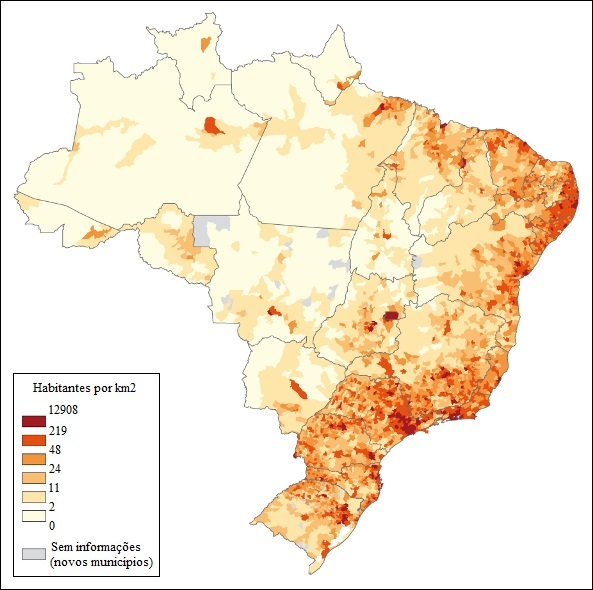
\includegraphics[scale=0.6]{coropletico-brasil.jpg}
\caption{Mapa coroplético (densidade demográfica). Fonte: \citet{wikicoropletico}.}
\label{coropletico}
\end{figure}
\end{comment}

São indicados para expor a distribuição das densidades (habitantes por quilômetro quadrado), rendimentos (toneladas por hectare), ou índices expressos em porcentagens os quais refletem a variação da densidade de um fenômeno (médicos por habitante, taxa de natalidade, consumo de energia) ou ainda, outros valores que sejam relacionados a mais de um elemento.

\subsection{Geoprocessamento}

Geoprocessamento é uma disciplina de estudo que visa unir conhecimentos tanto matemáticos quanto computacionais para tratar dados de origem espacial \citep{sig}. Dados espaciais (ou dados geográficos) são dados capazes de representar uma superfície terrestre e estão relacionados a determinada localização no espaço geográfico. O conjunto de dados espaciais tratados dá origem à informação geográfica, que por sua vez, é muito utilizada em diversas áreas, como Cartografia, Análise de Recursos Naturais, Transportes, Comunicações, Energia e Planejamento Urbano e Regional, com objetivo de melhorar o uso de recursos e entender fenômenos regionais variados \citep{introci}.

O Geoprocessamento é uma ferramenta bastante útil quando usada da maneira correta. Por exemplo, ao considerar um local de grande dimensão continental, com diversas divisões e regiões, pouco e muito desenvolvidas, porém com poucas informações estatísticas significativas para auxiliar nas decisões a serem tomadas sobre diversos problemas aplicados daquele local, o Geoprocessamento apresenta um enorme potencial, principalmente se baseado em tecnologias de custo relativamente baixo, em que o conhecimento seja adquirido localmente.

\citet{introci} faz menção a seguinte frase: “Se `onde' é importante para seu negócio, então Geoprocessamento é sua ferramenta de trabalho”. Nesta frase, o autor mostra que sempre que a variável ``onde'' existir dentre as questões e problemas que precisam ser resolvidos em determinado ambiente, um sistema gerido por Geoprocessamento é uma solução viável para esse objetivo.

\subsection{SIG}

As ferramentas computacionais para Geoprocessamento são chamadas de Sistemas de Informação Geográfica\footnote{em inglês, Geographic Information System (GIS).} (SIG). Elas permitem criar análises complexas, integrando dados de diversas fontes e possibilitando a criação bancos de dados georreferenciados \citep{sig}. 

Sistemas de Informação Geográfica se resumem basicamente a quatro atividades: coleta, gerenciamento, análise e disponibilização dos dados em um meio gráfico. Desta forma, é possível entender o que pertence a onde e analisar como os dados se relacionam uns com os outros. Mais do que nunca, esse tipo de ferramenta é primordial para resolver problemas complexos e baseados em localização.

Para \citet{geois}, os SIG, projetados para a entrada, o gerenciamento (armazenamento e recuperação), a análise e a saída de dados, devem ser utilizados em estudos nos quais a localização geográfica seja uma questão fundamental na análise, apresentando, assim, potencial para serem utilizados nas mais diversas aplicações.

A Figura \ref{arcgis} mostra um exemplo do SIG ArcGIS trabalhando com um mapa coroplético.% para análise de dados.

\begin{figure}[!h]
\centering
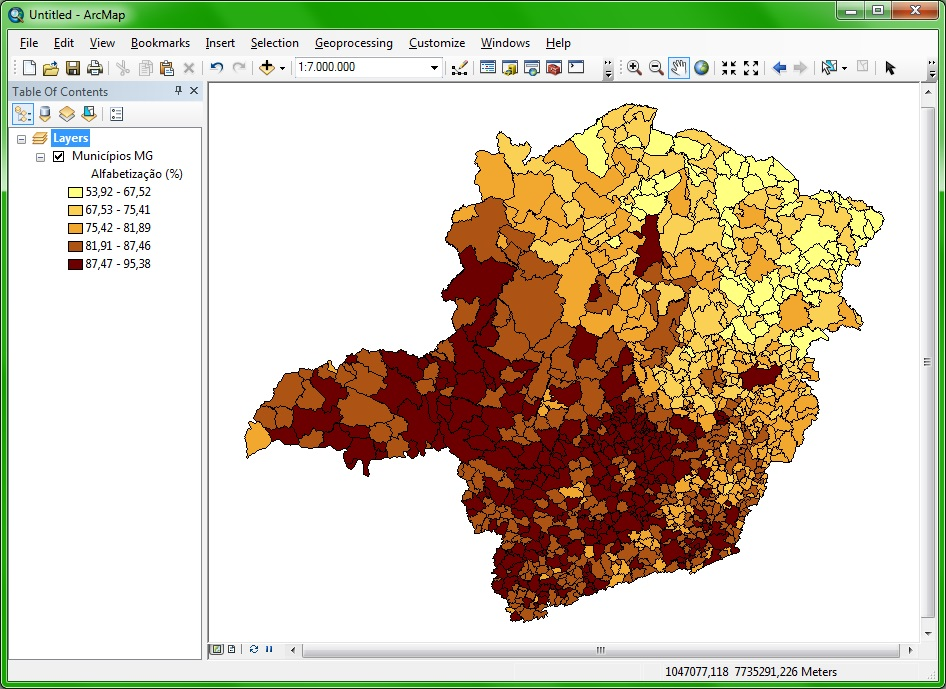
\includegraphics[scale=0.48]{ExemploArcGis.jpg}
\caption{ArcGIS utilizando mapa coroplético. Fonte: \citet{andersonm}.}
\label{arcgis}
\end{figure}

\subsection{API}

API (\emph{Application Program Interface})\footnote{em português, Interface de Programação de Aplicativos.} é um conjunto de rotinas, protocolos (padrões de programação) e ferramentas para criar aplicativos e softwares. Ela define um conjunto de operações que um aplicativo pode executar quando interage com o software. A API determina a funcionalidade que está disponível a um aplicativo, como também a dificuldade de se criar um programa para usar aquela funcionalidade \citep{redes}.

A maioria dos sistemas de programação define uma API dando um conjunto de procedimentos que o aplicativo pode chamar e os argumentos que cada procedimento espera. Normalmente, uma API contém um procedimento separado para cada operação básica \citep{redes}. Por exemplo, uma API poderia conter um procedimento que é usado para estabelecer uma comunicação e outro procedimento que é usado para enviar dados.

Existem muitos tipos diferentes de APIs para sistemas operacionais, aplicativos ou sites. O Windows, por exemplo, possui conjuntos de APIs que são usadas pelo hardware e aplicativos do sistema. Na \emph{Web} ela funciona como um serviço na qual uma aplicação faz uma requisição aos métodos e a API retorna um valor de resposta.

Segundo \citet{techtarget}, ``as APIs melhoraram fortemente a qualidade do software na última década e o crescente número de serviços da Web expostos através de APIs por provedores de nuvem também está encorajando a criação de aplicativos específicos para a nuvem, internet das coisas e aplicativos para suportar dispositivos móveis e usuários".

\subsection{D3.js}

D3 (Data-Driven Documents) é uma biblioteca de código aberto construída em JavaScript, desenvolvida para criar visualizações personalizadas e interativas de dados no navegador, fundamentada em cima de padrões comuns da \emph{Web} como HTML, CSS e SVG. Ela é capaz de interpretar e manipular bases de dados, gerando representações e recursos de interação \citep{d3}.

A ênfase da biblioteca é combinar técnicas de visualização e interação com uma abordagem orientada por dados para a manipulação de objetos do documento, dando-lhes as capacidades completas dos navegadores modernos e a liberdade de projetar a interface visual correta para seus dados. Ela conta com inúmeras formas de visualização e disposição de dados, dentre elas imagens, gráficos, calendários, diagramas, mapas, animações e outros, o que permite uma utilização de forma abrangente.

O diferencial do D3 é a manipulação eficiente de documentos com base em dados. \citet{d3} afirma que, com sobrecarga mínima, o D3 é extremamente rápido, suportando grandes conjuntos de dados e comportamentos dinâmicos para interação e animação. O estilo funcional do D3 permite a reutilização de código através de uma ampla coleção de módulos oficiais e desenvolvidos pela comunidade.

A Figura \ref{d3example} mostra exemplos de algumas formas de visualização de dados disponíveis na biblioteca D3.

\begin{figure}[!h]
\centering
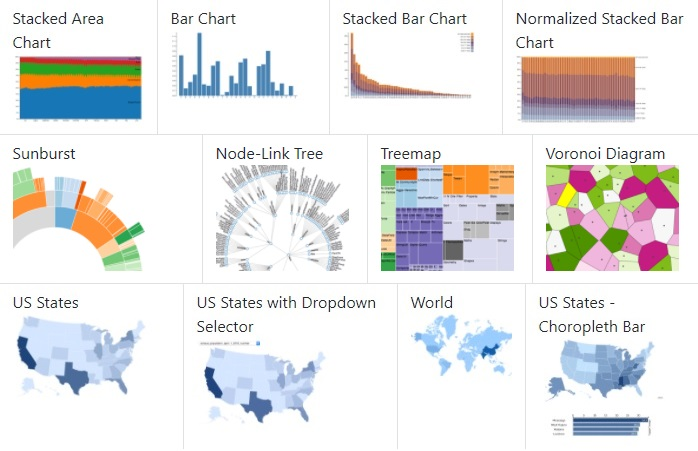
\includegraphics[scale=0.74]{d3-examples.jpg}
\caption{Exemplos de utilização de biblioteca D3. Fonte: \citet{d3}.}
\label{d3example}
\end{figure}

\section{Trabalhos Relacionados} \label{trabalhosre}

Nesta seção serão apresentados alguns trabalhos relacionados ao tema proposto.

\citet{cancado} apresentou uma tese que propunha um método que permitisse a realização de análises espaciais das interrupções no abastecimento de água do município de Belo Horizonte. Foram utilizados para a resolução do problema conceitos relacionados ao SIG, em especial as relações de proximidade e continência.

\citet{laudares} teve como objetivo em seu trabalho a investigação e classificação de componentes genéricos para Geovisualização na \emph{Web} e a organização de um ambiente virtual utilizado como repositório para dar suporte à geração de SIGs na Internet, comprovando a aplicabilidade e eficácia do uso desses componentes através da utilização em estudos de caso. \citeauthor{laudares} conclui que existe um aumento na utilização de componentes genéricos padronizados para o desenvolvimento de sistemas de Geovisualização, e afirma que o uso desses componentes no desenvolvimento de soluções para análise e visualização de dados espaciais visa atender os requisitos de padronização, uma vez que eles permitem que sistemas executados em diferentes ambientes que se comuniquem pelo mesmo padrão \emph{Web}.

\citet{santos} realizou em sua dissertação uma pesquisa que buscasse responder o seguinte problema: de que maneira a Representação Digital da Informação Geográfica (RDIG) na \emph{Web} colabora para a construção do conhecimento cientifico? Trata-se de uma pesquisa de nível exploratório e descritivo, onde foram utilizados registros bibliométricos como fontes de dados e métodos cientométricos para a coleta e a análise dos dados. Utilizou também o \emph{software VOSViewer} para visualização do mapa de termos, fazendo uso da metáfora de distância utilizados em mapas tradicionais para representar os relacionamentos entre os termos. \citeauthor{santos} conclui que houve uma tendência de crescimento da quantidade de trabalhos acadêmicos relacionados ao RDIG, o que sustenta a hipótese de colaboração deste meio à construção do conhecimento científico.

\citet{kutova} desenvolveu uma biblioteca (GeoPUCMinas) com recursos em JavaScript para a produção de mapas e para análises espaciais do estado de Minas Gerais. Com o objetivo de análise espacial dos cursos superiores e das matrículas nesses cursos nos municípios do estado de Minas Gerais, \citeauthor{kutova} também desenvolveu o Mapeamento da Educação Superior (MAPES), que integrado a essa biblioteca, era possível obter várias formas de representação de dados, como mapas e gráficos, do Censo Demográfico 2010 do IBGE\footnote{Instituto Brasileiro de Geografia e Estatística.} e do Censo de Educação Superior 2010 do INEP\footnote{Instituto Nacional de Estudos e Pesquisas Educacionais Anísio Teixeira.}.

\citet{magno}, como extensão do trabalho realizado por \citet{kutova}, utilizou a biblioteca GeoPUCMinas e a modificou a ponto que permitisse que o usuário inserisse sua própria base de dados com informações sobre os municípios de Minas Gerais. Além disso, desenvolveu funcionalidades que permitissem personalizar a apresentação do mapa, como inserção de título e definição de intervalos das classes.

Como complemento dos trabalhos de \citet{kutova} e \citet{magno}, o diferencial deste projeto se dá pelo desenvolvimento de uma nova API com tecnologia \emph{open source}, passível de vinculação a qualquer página \emph{Web}, contendo funções para criação e personalização de mapas que viabilizam o seu uso em relação aos SIGs. Além disso, a API irá maximizar o seu uso pois deixará de ser restrita apenas ao estado de Minas Gerais, ou seja, será possível trabalhar com dados municipais de qualquer área do território brasileiro (de regiões à microrregiões). %necessitando apenas da inserção uma base de dados referente, obtendo assim, estruturas contendo informações concretas para análise dos mesmos.

\section{Metodologia} \label{metodologia}

Este trabalho apresenta o desenvolvimento de uma API com funções para desenhos, configuração e manipulação de dados espaciais municipais por meio de uma mapa coroplético.

\subsection{Etapas da Pesquisa} \label{atividades}

A metodologia para construção e definição da API será divida nas seguintes etapas, conforme a Figura \ref{fluxograma}:

\begin{figure}[!h]

\centering

\tikzstyle{block} = [rectangle, draw, rounded corners, inner sep=2mm, text centered, minimum height=4em]
\tikzstyle{line} = [draw, -latex']
    
\begin{tikzpicture}[node distance=0.5cm, >=stealth, auto]
	\scalefont{0.9}
    \node [block, text width=2.2cm] (requisitos) {Levantamento de requisitos};
    \node [block, right=of requisitos, text width=1.9cm] (modelagem) {Modelagem do sistema};
    \node [block, right=of modelagem, text width=2.7cm] (desenvolvimento) {Desenvolvimento da API};
    \node [block, right=of desenvolvimento, text width=1.2cm] (teste) {Teste da API};
    \node [block, right=of teste, text width=1.8cm] (avaliacao) {Avaliação dos resultados};
    \path [line] (requisitos) -- (modelagem);
    \path [line] (modelagem) -- (desenvolvimento);
    \path [line] (desenvolvimento) -- (teste);
    \path [line] (teste) -- (avaliacao);
\end{tikzpicture}

\caption{Fluxograma com as etapas da metodologia de desenvolvimento API.}
\label{fluxograma}
\end{figure}

\begin{enumerate}[I]
  \item{Levantamento de requisitos;}  
  \item{Modelagem do sistema;}
  \item{Desenvolvimento da API;}  
  	\begin{enumerate}
    	\item{Criação e leitura da base de mapas brasileiros;}  
        \item{Métodos para desenho poligonal;}  
        \item{Métodos para inserção de dados e configuração de exibição;} 
    	\item{Desenvolvimento da aplicação \emph{Web} de teste;} 
  	\end{enumerate}
  \item{Teste da API;}  
  \item{Avaliação dos resultados.}
\end{enumerate}

No levantamento de requisitos foi feita uma análise %junto aos professores Dr. Marcos André Silveira Kutova (diretor de Ensino a Distância da PUC Minas) e Dr. Paulo Fernando Braga Carvalho (coordenador do Curso de Pós-Graduação em Geoprocessamento e Análise Espacial da PUC Minas), 
com o objetivo de levantar quais as características e funcionalidades necessárias à API, informações sobre o tipo de dados e sua origem, além de outras informações voltadas ao sistema (requisitos não funcionais).

Na etapa de modelagem do sistema foi elaborado um diagrama de casos de uso, com propósito de facilitar o processo de desenvolvimento da aplicação.

O desenvolvimento do sistema foi a etapa onde houve a construção efetiva da API e da aplicação teste. Foi preciso avaliar as tecnologias disponíveis e selecionar aquelas que melhor se adequavam aos requisitos. A subseção \ref{tecnologias} explicitará melhor essa análise.

O teste da API consistiu, por meio da aplicação teste, em validar as funções de carga de arquivo de dados, desenho de polígonos e configuração do mapa.

%Na etapa de teste de usabilidade do sistema, o mesmo foi submetido à algumas pessoas na qual este sistema seria interessante. Assim, foi construído um questionário e aplicado a elas, com questões referentes as funcionalidades e usabilidade do sistema.

Na etapa de avaliação dos resultados foi feita uma análise do teste, levando em consideração o funcionamento dos recursos disponibilizados pela API.

\subsection{Ambiente de Desenvolvimento} \label{tecnologias}

Para desenvolver a API com as características necessárias para este trabalho, foi preciso avaliar as tecnologias atuais para encontrar as que mais se adequavam ao projeto. Essa avaliação foi realizada em três etapas, conforme descrito a seguir.

A primeira etapa refere-se a definição de uma plataforma de visualização de dados. Essa plataforma deve permitir visualizar dados tanto de áreas maiores, como países e estados, quanto menores, como regiões metropolitanas e municípios, sendo que estes dados devem ser impressos sobre um mapa coroplético. Desta maneira, foi utilizada a biblioteca D3. Com ela foi possível criar mapas temáticos e interativos.

A segunda etapa refere-se ao tipo de arquivo de mapas. Foi preciso observar a compatibilidade do arquivo com a plataforma de visualização e como são representados os objetos gráficos no tipo de arquivo (pontos, linhas, polígonos, altitude, longitude, etc.). O formato que mais atendeu aos requisitos foi o TopoJSON, uma simplificação GeoJSON, tanto em informações quanto no tamanho do arquivo, sendo eficaz para este projeto e compatível com a biblioteca D3. %A API ainda suportará arquivos nos formatos GeoJson e Shapefile, pois os mesmos poderão ser convertidos pela API para o formato TopoJson. Para fazer a leitura dos arquivos e realizar as conversões, será utilizado o npm, um gerenciador de pacotes da biblioteca Node.js. Ele é capaz de buscar e importar pacotes necessários na aplicação, fazendo as atualizações quando necessárias.

A terceira etapa consistiu na definição do tipo de arquivo que conteria os dados a serem visualizados. Foi escolhido o formato CSV, por ser de fácil utilização e acessível a qualquer usuário. Esses dados, após carregados na API, são tratados, convertidos em JSON e feito as aplicações ao mapa.

Outro ponto essencial deste projeto é o desenvolvimento de uma aplicação teste. Esta aplicação foi desenvolvida para testar e validar a API, utilizando padrões \textit{Web}, como HTML, CSS e JavaScript.

Todo o projeto foi desenvolvido através do Visual Studio Code\footnote{Visual Studio Code: \href{https://code.visualstudio.com/download}{https://code.visualstudio.com/download}}, um moderno editor de código fonte, compatível com diversas linguagens de programação.%juntamente com o software XAMPP, que emula um servidor local para realização dos testes.

A Tabela \ref{tabtecnologias} apresenta um resumo das tecnologias e recursos utilizados.

\begin{table}[!htbp]
	\centering
    \caption{Ferramentas do ambiente de desenvolvimento}
	\begin{tabular}{|c|c|}
    \hline
    \multicolumn{1}{|c|}{{\cellcolor[rgb]{.75, .75, .75} \textbf{Funcionalidades}}} & \multicolumn{1}{|c|}{{\cellcolor[rgb]{.75, .75, .75} \textbf{Ferramentas}}}
    \tabularnewline \hline  
      Desenvolvimento & Visual Studio Code \tabularnewline \hline
      Formato dos arquivos de mapas & TopoJSON \tabularnewline \hline
      Formato dos dados & CSV e JSON \tabularnewline \hline
      Plataforma de visualização de dados & D3.js \tabularnewline \hline
      Programação \emph{Web} & HTML, CSS e JavaScript \tabularnewline \hline
      Recursos auxiliares (JavaScript) & jQuery, GeoStat e Numeral \tabularnewline \hline
      Sistema operacional & Windows 10 \tabularnewline \hline
%      Gerenciador de pacotes & Node.js (npm) \tabularnewline \hline
	\end{tabular}
    \label{tabtecnologias}
\end{table} 

\begin{comment}

\subsection{Cronograma}

Para realização das atividades já referenciadas na subseção \ref{atividades}, foi proposto um cronograma de acordo com o tempo previsto de execução de cada uma, apresentado na Tabela \ref{tabcronograma}.

%\begin{table}[htbp]
%	\centering
%   \caption{Cronograma de atividades}
%	\begin{tabular}{|c|c|c|c|c|c|c|}
%      \hline
%      \multicolumn{1}{|c|}{\multirow{2}[4]{*}{\textbf{Atividades}}} & \multicolumn{6}{c|}{\textbf{Período}} \tabularnewline 
%      \cline{2-7} & \textbf{Jun/17} & \textbf{Jul/17} & \textbf{Ago/17} & \textbf{Set/17} & \textbf{Out/17} & \textbf{Nov/17} \tabularnewline \hline
%      I 	& \cellcolor[rgb]{.75, .75, .75}x x x &  &  &  &  & \tabularnewline \hline
%      II 	& \cellcolor[rgb]{.75, .75, .75}x x x &  &  &  &  & \tabularnewline \hline
%      III-a &  & \cellcolor[rgb]{.75, .75, .75}x x x &  &  &  & \tabularnewline \hline
%      III-b &  & \cellcolor[rgb]{.75, .75, .75}x x x & \cellcolor[rgb]{.75, .75, .75}x x x &  &  & \tabularnewline \hline
%      III-c &  &  & \cellcolor[rgb]{.75, .75, .75}x x x & \cellcolor[rgb]{.75, .75, .75}x x x &  & \tabularnewline \hline
%      III-d &  &  &  & \cellcolor[rgb]{.75, .75, .75}x x x &  & \tabularnewline \hline
%      IV 	&  &  &  &  & \cellcolor[rgb]{.75, .75, .75}x x x & \tabularnewline \hline
%      V 	&  &  &  &  & \cellcolor[rgb]{.75, .75, .75}x x x &  \tabularnewline \hline
%      VI 	&  &  &  &  &  & \cellcolor[rgb]{.75, .75, .75}x x x \tabularnewline \hline
%	\end{tabular}
%    \label{tabcronograma}
%\end{table}

\begin{table}[!htbp]
	\scalefont{0.8}
	\centering
    \caption{Cronograma de atividades}
	\begin{tabular}{|>{\centering\arraybackslash}m{0.7cm}|>{\arraybackslash}m{5cm}|>{\centering\arraybackslash}m{0.9cm}|>{\centering\arraybackslash}m{0.9cm}|>{\centering\arraybackslash}m{0.9cm}|>{\centering\arraybackslash}m{0.9cm}|>{\centering\arraybackslash}m{0.9cm}|>{\centering\arraybackslash}m{0.9cm}|}
     \hline
     \multicolumn{1}{|c|}{\multirow{2}{*}{\textbf{Item}}} & \multicolumn{1}{c|}{\multirow{2}{*}{\textbf{Atividades}}} & \multicolumn{6}{c|}{\textbf{Período}} \\
     \cline{3-8} & & \textbf{Jun/17} & \textbf{Jul/17} & \textbf{Ago/17} & \textbf{Set/17} & \textbf{Out/17} & \textbf{Nov/17} \\ \hline
      I & Levantamento de requisitos & \cellcolor[rgb]{.75, .75, .75}x x x &  &  &  &  & \\ \hline
      II & Modelagem do sistema & \cellcolor[rgb]{.75, .75, .75}x x x &  &  &  &  & \\ \hline
      III-a & Criação e leitura da base de mapas brasileiros &  & \cellcolor[rgb]{.75, .75, .75}x x x &  &  &  & \\ \hline
      III-b & Métodos para desenho poligonal &  & \cellcolor[rgb]{.75, .75, .75}x x x & \cellcolor[rgb]{.75, .75, .75}x x x &  &  & \\ \hline
      III-c & Métodos para inserção de dados e configuração de exibição; &  &  & \cellcolor[rgb]{.75, .75, .75}x x x & \cellcolor[rgb]{.75, .75, .75}x x x &  & \\ \hline
      III-d & Desenvolvimento da aplicação \emph{Web} de teste &  &  &  & \cellcolor[rgb]{.75, .75, .75}x x x &  & \\ \hline
      IV & Teste do sistema &  &  &  &  & \cellcolor[rgb]{.75, .75, .75}x x x & \\ \hline
      V & Teste de usabilidade do sistema &  &  &  &  & \cellcolor[rgb]{.75, .75, .75}x x x & \\ \hline
      VI & Apresentação e análise dos resultados &  &  &  &  &  & \cellcolor[rgb]{.75, .75, .75}x x x \\ \hline
	\end{tabular}
    \label{tabcronograma}
\end{table}

% \cellcolor[rgb]{1, .753, 0} 

Pretende-se ao término do segundo semestre de 2017 realizar a apresentação do projeto em pleno funcionamento, testado e validado. Posteriormente, será possível disponibilizar a plataforma para o uso acadêmico em pesquisas e rotinas de estudos.

\end{comment}

\section{Desenvolvimento} \label{desenvolvimento}

Nesta seção serão apresentados artefados gerados com o desenvolvimento.

Para acesso e download da API, a mesma pode ser encontrada através do \textit{link} \href{https://paulofernando.mat.br/geomapbr/}{https://paulofernando.mat.br/geomapbr/}.

\subsection{Levantamento de Requisitos}

Após análise das necessidades do sistema, foram definidos os requisitos necessários.

Para os requisitos funcionais, as funcionalidades da API devem garantir ao sistema:

\begin{itemize}
\item RF01: permitir ao usuário inserção de dados;
\item RF02: permitir ao usuário identificação dos campos a serem representados (identificador do registro [opcional], código do município [obrigatório], descritor do registro [opcional] e valor do atributo [obrigatório]);
\item RF03: permitir ao usuário escolher o tipo de operação desejada (contagem, média ou soma);
\item RF04: permitir ao usuário alterar configurações de classificação (método, número de classes, casas decimais e coloração);
\item RF05: permitir ao usuário escolha das bordas territoriais que deseja aplicar ao mapa;
\item RF06: permitir ao usuário aplicação de filtros por áreas do território brasileiro (região, estado, mesorregião e microrregião);
\item RF07: permitir ao usuário representar dados espaciais no mapa;
\item RF08: permitir ao usuário visualizar séries temporais.
\end{itemize}

Para os requisitos não funcionais, a API deve:

\begin{itemize}
\item RNF01: manter os dados espaciais salvos durante toda a configuração e reconfiguração;
\item RNF02: ser \emph{Web}.
\end{itemize}

\subsection{Modelagem do Sistema}

A Figura \ref{casosdeuso} mostra as interações do sistema com as funcionalidades e métodos fornecidos pela API.

\begin{figure}[!h]
\centering
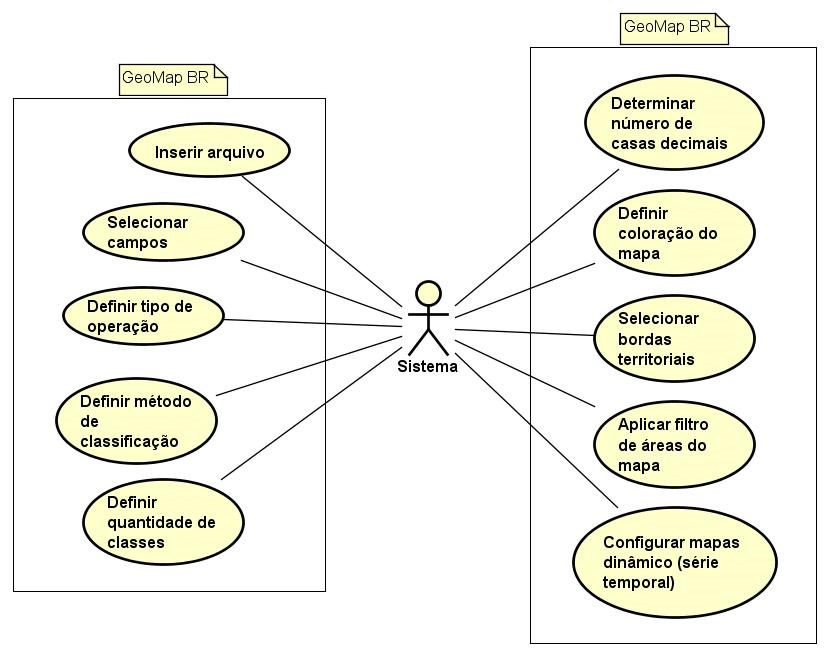
\includegraphics[scale=0.51]{casosdeuso.jpg}
\caption{Diagrama de caso de uso. Fonte: Elaborada pelo autor.}
\label{casosdeuso}
\end{figure}

\subsection{Funcionalidades da API}

O propósito da API é fornecer um mecanismo de geração de um mapa coroplético brasileiro interativo, capaz de receber dados e os transcrevê-los na forma de classes de cores, e que tenha propriedades para configuração de visualização. Para tanto, foram criadas funções e métodos com as seguintes funcionalidades:

\begin{itemize}
\item geração de um mapa;
\item inserção de arquivo de dados CSV, separados por vírgula, ponto e vírgula, barra vertical ou tabulação;
\item seleção e inserção dos nomes dos campos necessários para classificação e exibição dos dados;
\item definição do tipo de operação para análise dos dados (contagem, média ou soma);
\item definição do método a ser utilizado na classificação dos dados (intervalos iguais, intervalos manuais, quantis ou quebras naturais);
\item definição da quantidade de classes;
\item definição do número de casas decimais para arredondamento dos dados;
\item definição e inversão da escala de cores;
\item exibição personalizada das bordas limítrofes (região, estado, mesorregião, microrregião e município);
\item aplicação de filtro personalizado (região, estado, mesorregião ou microrregião);
\item classificação dos dados baseados na massa de dados ou no filtro aplicado;
\item exibição e configuração de mapa dinâmico (série de dados em visualização temporal).
\end{itemize}

Para um maior detalhamento das funcionalidades, encontra-se acessível em \href{https://paulofernando.mat.br/geomapbr/api.html}{https://paulofernando.mat.br/geomapbr/api.html} uma documentação com a descrição de todos métodos e funções disponibilizados na API.

\section{Teste da API} \label{teste}

A API GeoMap BR foi desenvolvida utilizando JavaScript, tendo como principal biblioteca a D3.js\footnote{D3.js: \href{https://d3js.org/}{https://d3js.org/}}. Ela conta também com o acoplamento de outras bibliotecas em seu desenvolvimento, sendo estas jQuery\footnote{jQuery: \href{https://jquery.com}{https://jquery.com}}, GeoStats\footnote{GeoStats: \href{https://github.com/simogeo/geostats}{https://github.com/simogeo/geostats}} e Numeral\footnote{Numeral: \href{https://numeraljs.com/}{https://numeraljs.com/}}. Para testá-la, foi desenvolvida uma aplicação que pode ser acessada pelo link \href{https://paulofernando.mat.br/geomapbr/app.html}{https://paulofernando.mat.br/geomapbr/app.html}.

Para acessar a API, é preciso vincular a mesma à aplicação desenvolvida. Deve-se fazer o download desta, extraí-la na pasta raíz do projeto, e na página onde será gerado o mapa, deve-se fazer a inclusão dos arquivos necessários, conforme exemplo abaixo.

\begin{lstlisting}
<script src="https://code.jquery.com/jquery-3.2.1.min.js"></script>       
<script src="https://d3js.org/d3.v3.min.js"></script>
<script src="https://d3js.org/topojson.v1.min.js"></script>
<script src="https://d3js.org/queue.v1.min.js"></script>
<script src="geomapbr/js/geomapbr.js"></script>
<script src="geomapbr/js/geostats.min.js"></script>
<script src="https://cdnjs.cloudflare.com/ajax/libs/numeral.js/2.0.6/numeral.min.js"></script>
<link rel=stylesheet href="geomapbr/css/geomapbr.css">
\end{lstlisting}

O primeiro passo para utilizar a API é criar uma instância da classe geoMapBR, que dará acesso aos métodos para criação, manipulação e configuração do mapa. Na página é necessário um elemento DIV (com largura e altura definidos) onde será desenhado o mapa. O código abaixo mostra como deve ser feita a instanciação da classe, sendo o parâmetro do construtor, o id do elemento DIV criado.

\begin{lstlisting}
var gmb;
gmb = new geoMapBR("id_div");
\end{lstlisting}

Para carregar o mapa é necessário a chamada do método \textit{gerarMapa()}. Este faz algumas verificações de variáveis de configuração e chama outros métodos responsáveis pelo desenho dos polígonos e áreas. O código a seguir mostra a chamada do método e a Figura \ref{mapaVazio} o resultado da operação, sendo um mapa vazio, já que não foram setados dados.

\begin{lstlisting}
gmb.gerarMapa();
\end{lstlisting}

\begin{figure}[h]
\centering
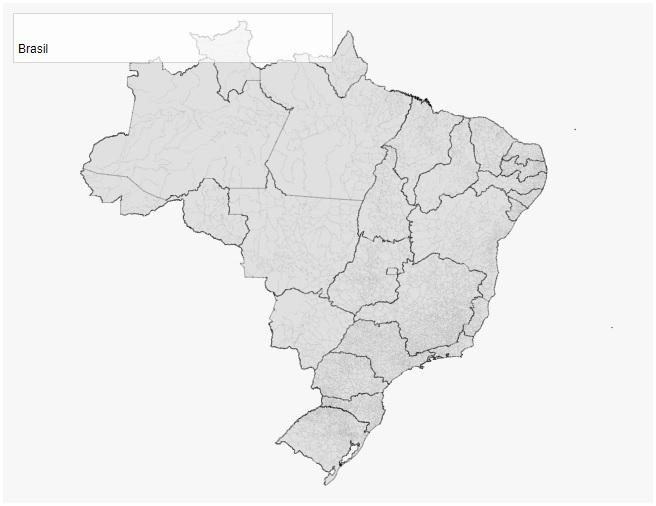
\includegraphics[scale=0.65]{mapa-branco.jpg}
\caption{Mapa sem dados.}
\label{mapaVazio}
\end{figure}

Para representar os dados relacionados ao território brasileiro, é necessário um arquivo CSV. Para este teste foi utilizado o modelo representado na Figura \ref{baseDados}. A primeira coluna do modelo trata-se do identificador do registro, a segunda coluna o código do município (IBGE), e as demais colunas representam atributos que serão representados no mapa.

\begin{figure}[!h]
\centering
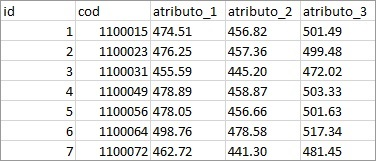
\includegraphics[scale=1]{base-de-dados.jpg}
\caption{Arquivo CSV.}
\label{baseDados}
\end{figure}

O método \textit{setDados(arquivo, callback)} é responsável por carregar um arquivo de dados à API. Ele recebe como parâmetro o arquivo de dados, obtido por meio do elemento HTML ``input file", e uma função de callback que será executada após a leitura completa do arquivo. O método \textit{getAtributos()} retorna um \textit{array} de \textit{string} contendo o nomes dos campos do arquivo. Ele deve ser colocado dentro da função de callback do método \textit{setDados} para garantir que a leitura dos dados já esteja finalizada no momento da chamada deste método, conforme o código a seguir.

\begin{lstlisting}
gmb.setDados(
  document.getElementById("id_input_file").files, function(){
    atributos = gmb.getAtributos();
  });
});
\end{lstlisting}

Para gravar os campos escolhidos da base de dados, a API possui métodos para setar estes valores, sendo necessários o campo com o código do município, o campo com o valor, o campo com o identificador do registro (opcional) e o campo com a descrição do registro (opcional). Todos estes métodos recebem como parâmetro uma \textit{string} com o nome do campo, conforme o código abaixo.

\begin{lstlisting}
gmb.setCampoId("id");
gmb.setCampoCodMunicipio("cod");
gmb.setCampoValor("atributo_1");
\end{lstlisting}

Quanto a operação com os dados, a API é capaz de realizar contagem de registros, média dos valores ou soma dos mesmos. O exemplo abaixo define o tipo de operação de dados como média.

\begin{lstlisting}
gmb.setOperacaoMedia();
\end{lstlisting}

A configuração do mapa permite a manipulação da forma com que os dados serão apresentados. Nesta configuração, é possível informar, como por exemplo, o método que será utilizado para a classificação de dados (intervalos iguais, intervalos manuais, quantis, ou quebras naturais), o número de classes que serão divididos os dados, e o esquema de cores para coloração do mapa (azul, laranja, roxa, verde, vermelha e espectral). O código abaixo define o método de classificação sendo como quebras naturais, quantidade de classes como cinco, e o esquema de cores como vermelho. É gerado novamente o mapa para realizar a aplicação das configurações setadas. O resultado é representado na Figura \ref{mapaCarregado}.

\begin{lstlisting}
gmb.setMetodoQuebrasNaturais();
gmb.setQtdClasses(5);
gmb.setCorVermelha();
gmb.gerarMapa();
\end{lstlisting}

\begin{figure}[!h]
\centering
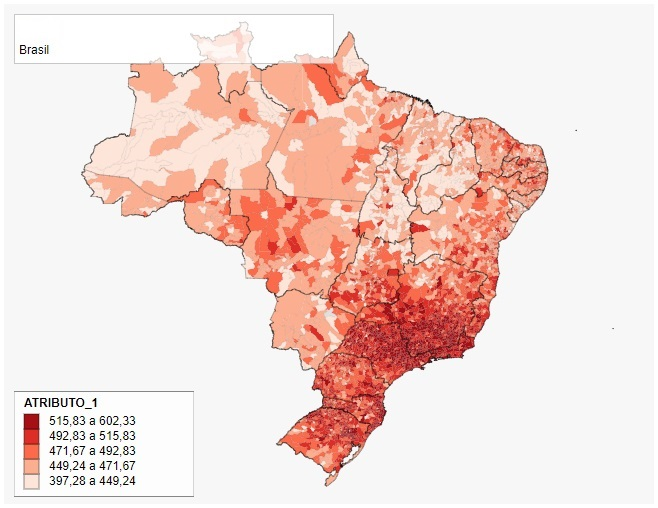
\includegraphics[scale=0.65]{mapa-carregado.jpg}
\caption{Mapa com dados carregados.}
\label{mapaCarregado}
\end{figure}

Em cada município do mapa, é possível clicar sobre o mesmo e obter informações quanto a sua localização por meio de uma janela de informações. Quando já há dados carregados, também é possível visualizar os atributos que estão vinculados àquele local, como mostra a Figura \ref{mapaInfo}.

\begin{figure}[!h]
\centering
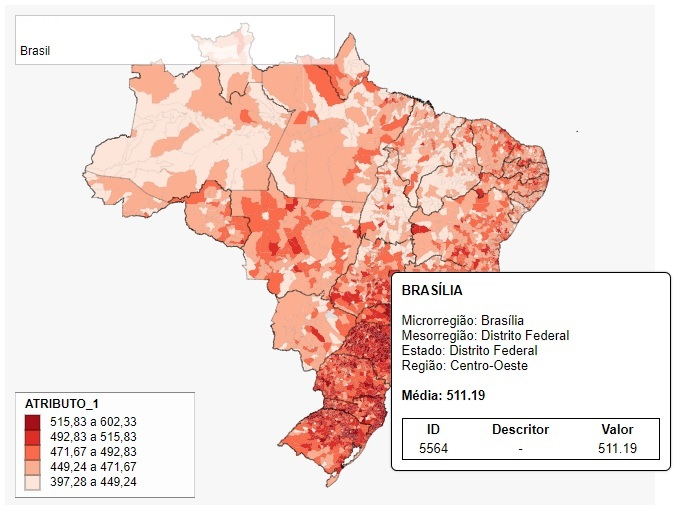
\includegraphics[scale=0.6]{mapa-info.jpg}
\caption{Janela de informação.}
\label{mapaInfo}
\end{figure}

A API possui uma funcionalidade que permite setar quais as bordas limítrofes serão desenhadas no mapa. Elas podem ser de regiões, estados, mesorregiões, microrregiões e/ou municípios. Por padrão, o mapa é desenhado com bordas de municípios e estados. Os métodos responsáveis por isso devem receber um parâmetro booleano, ou seja, \textit{true} para desenhar as bordas ou \textit{false} para ocultá-las. O código a seguir exemplifica esta funcionalidade, limpando as bordas ativas e setando para que sejam desenhadas as bordas de regiões e mesorregiões. Também é alterado a coloração do mapa  para verde. O resultado é mostrado na Figura \ref{mapa-bordas}.

\begin{lstlisting}
gmb.setDesenhaBordaMunicipio(false);
gmb.setDesenhaBordaMesorregiao(true);
gmb.setDesenhaBordaEstado(false);
gmb.setDesenhaBordaRegiao(true);
gmb.setCorVerde();
gmb.gerarMapa();
\end{lstlisting}

\begin{figure}[!h]
\centering
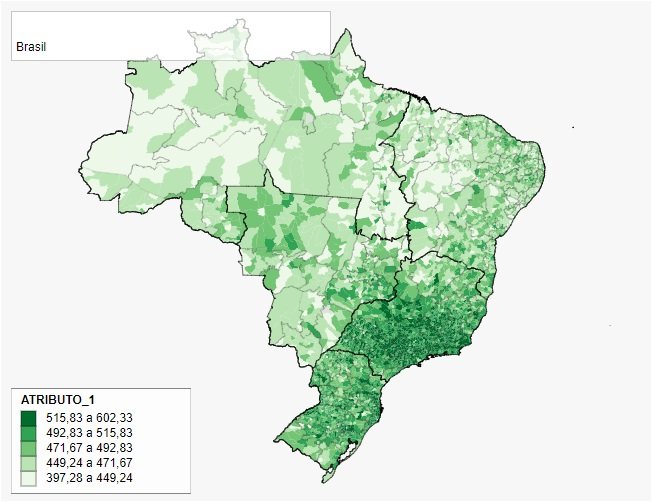
\includegraphics[scale=0.63]{bordas-regiao-meso.jpg}
\caption{Mapa com bordas de região e mesorregião.}
\label{mapa-bordas}
\end{figure}

Outra funcionalidade é aplicação de filtro sobre o mapa. Ele permite que apenas uma área especifica seja impressa, por exemplo, a mesorregião Metropolitana de Belo Horizonte. Os filtros disponíveis são de região, estado, mesorregião e microrregião. O parâmetro de cada um destes métodos é o código da área desejada (segundo IBGE). O código abaixo mostra a aplicação do filtro de região, passando como parâmetro o código '3', referente à região Sudeste. A Figura \ref{mapaRegiao} representa o resultado esta ação.

\begin{lstlisting}
gmb.setFiltroRegiao(3);
gmb.gerarMapa();
\end{lstlisting}

\begin{figure}[!h]
\centering
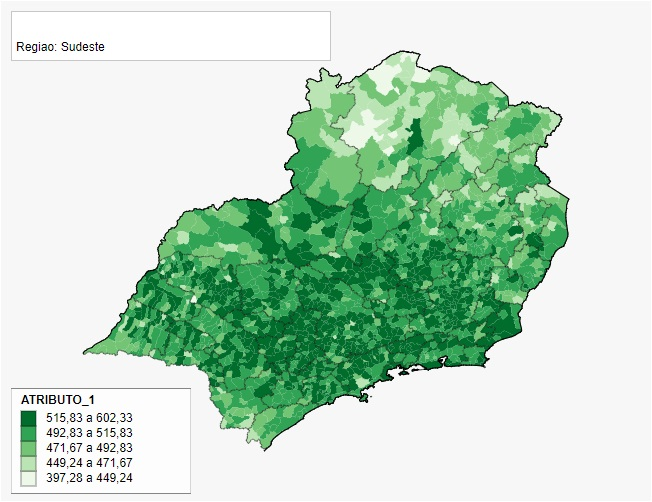
\includegraphics[scale=0.63]{regiao.jpg}
\caption{Filtro sobre a região Sudeste.}
\label{mapaRegiao}
\end{figure}

Uma última funcionalidade implementada na API é um recurso que permite gerar mapas dinâmicos, ou seja, ao invés de mostrar no mapa um atributo fixo, a API percorre o arquivo de dados, mostrando automaticamente, de tempo em tempo, um atributo diferente, sequencialmente. Para tanto, é preciso ativar o mapa dinâmico, setar um tempo em segundos para a transição entre os atributos e configurar se ao término dos campos a API entrará em \textit{loop} e reiniciará a apresentação dos atributos ou se finalizará. O código abaixo mostra a ativação do mapa dinâmico, atribuição do tempo de transição em cinco segundos e a interrupção da apresentação dos dados ao término dos atributos.  

\begin{lstlisting}
gmb.setSerieTemporalAtivar(true);
gmb.setSerieTemporalTempo(5);
gmb.setSerieTemporalLoop(false);
gmb.gerarMapa();
\end{lstlisting}

Finalizado os testes acima, foram validadas as principais funções e métodos disponibilizados pela API, comprovando o aninhamento de seu objetivo com as funcionalidades providas. Outras funções estão disponíveis, como, por exemplo, métodos \textit{get} de todas as funcionalidades testadas. Para conhecer o uso destes e de outros métodos, foi elaborado um tutorial mais aprofundado que está disponível em \href{https://paulofernando.mat.br/geomapbr/tutorial.html}{https://paulofernando.mat.br/geomapbr/tutorial.html}.

\begin{comment}

\section{Sem Nome} \label{teste}

Para configuração e personalização do mapa, foi elaborado uma tela para o usuário identificar estes aspectos, conforme a Figura \ref{telaConfiguracao}. Estas opções são a inclusão de um título ao mapa, entrada de dados, identificação dos campos do arquivo inserido, definição da operação que será realizada com os valores por município (contagem, média ou soma), seleção de método que será utilizado para classificação e agrupamento dos dados (intervalos iguais, intervalos manuais, quantis ou quebras naturais), definição da quantidade de classes e número de casas decimais para arredondamento dos valores, escolha do esquema de cores a ser aplicado, opção de inversão da tonalidade das cores, opção de classificação de acordo com a massa de dados ou o filtro selecionado, seleção de divisões regionais que serão desenhadas no mapa, aplicação de filtro por área e configuração de mapa dinâmico.

\begin{figure}[!h]
\centering
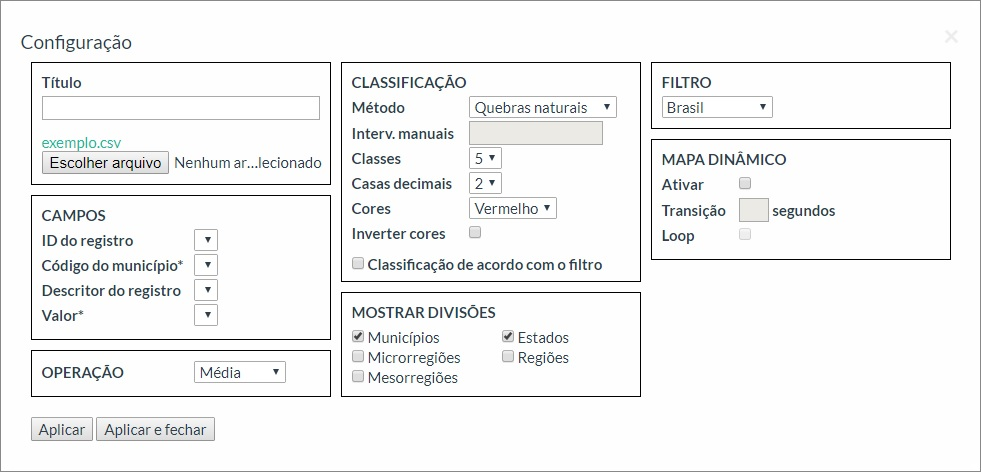
\includegraphics[scale=0.55]{configuracoes-mapa.jpg}
\caption{Tela de configuração do mapa. Fonte: Elaborada pelo autor.}
\label{telaConfiguracao}
\end{figure}

\end{comment}

\section{Conclusão} \label{conclusao}

Este trabalho apresentou o desenvolvimento de uma API \emph{Web} que permitisse a análise espacial de dados municipais do território brasileiro por meio da geovisualização em um mapa coroplético, bem como uma aplicação para avaliação e testes destes recursos. O download da API, acesso à documentação, ao tutorial e à aplicação teste, encontram-se disponíveis em \href{https://paulofernando.mat.br/geomapbr/}{https://paulofernando.mat.br/geomapbr/}. 

Neste desenvolvimento, foram testadas as funcionalidades criadas para a API. Os resultados mostram o pleno funcionamento e a compatibilidade dos métodos desenvolvidos com os requisitos levantados na análise do desenvolvimento da API. A API foi capaz de receber uma carga de dados e realizar operações, permite setar configurações de exibição dos dados no mapa de forma a facilitar a compreensão dos mesmos, além de conseguir gerar progressões temporais dinâmicas com os dados. O tempo de resposta da API é outro ponto interessante, pois tanto a leitura dos dados quanto o desenho dos mapas são feitos de forma rápida.

A principal contribuição deste trabalho foi a criação de uma ferramenta que pode ser incorporada à qualquer página \emph{Web}, possibilitando o trabalho e a análise de mapas e dados brasileiros independente de se ter e/ou conhecer um SIG.

Como trabalhos futuros pretende-se trabalhar com dados não apenas municipais, mas abranger para os demais níveis territoriais (região, estado, mesorregião e microrregião). Além disso, pode ser trabalhado na API uma forma de gerar impressão de mapas, extração da exibição dinâmica em formato de vídeos, e criar outras formas gráficas para analisar os dados juntamente com o mapa, como gráficos de barras e dispersão.%, com opção de selecionar as variáveis a ser representadas nos eixos.

\newpage

\bibliographystyle{apa}
\bibliography{referencias}

\end{document}